\documentclass[a4j,12pt]{jarticle}
\usepackage[dvipdfmx]{graphicx}
\usepackage{amssymb}
\usepackage{amsmath}
\usepackage{float}
\usepackage{url}
\begin{document}
\begin{center}
\thispagestyle{empty}
\vspace*{5zh}
\huge
令和2年度 卒業論文\\[50pt]
{\Huge 論理的文章のアウトラインの作成を

支援するツールの開発}\\
[80pt]
\huge
指導教員 須田 宇宙 准教授\\[30pt]
千葉工業大学 情報ネットワーク学科\\[10pt]
須田研究室\\[60pt]
1632144 \hspace{70pt} 三浦 恋\\[75pt]
\end{center}
\vspace*{-2cm}
\begin{flushright} 
\huge
提出日 2020年1月--日
\end{flushright}

\newpage
\pagenumbering{roman}
\tableofcontents
\newpage
\pagenumbering{arabic}
\section{緒言}
%目次を作る際は\verb+\tableofcontents+ と打ちます。\\
%新しいページに区切るときは\verb+\newpage+ と打ちます

%背景
大学生に対して,論理的な思考力や論理的文章作成能力の要求が高まっている.
しかし,論文やレポートを書く際にアウトラインなどの事前準備をせずに文章の作成を行ってしまう学生が多く,論理的な文章にならないことが問題点として挙げられる.
そのため,レポートの書き方の指導や修正を行うライティングセンターの設置などが進められているが
自発的に利用しなければ文章作成力は向上しない.

%問題点
一般に論文や小説などの長文を作成するためのツールとして,アウトラインプロセッサが使用されることが多い.
これは,文章を階層的に管理することに主眼が置かれており,学生にとって主張や根拠などが明確な一貫した文章を書く力を養うためのツールではないことが問題点となっている.

%目的
そこで本研究では,主張や根拠などが明確な一貫した文章を書く力を身に付け,論文やレポートの作成を支援するアカデミックアウトラインツールを開発することを目的としている.
\newpage
\section{アカデミックライティングについて}
本章では論文やレポートについて説明をする.
\subsection{論文とは}
論文とはエッセイや小説のように自由な文章表現ではなく,一定の形式に備えた文章表現である.またテーマをもとに問題をたて,問題に対し様々な手法で,分析,考察し問題解決につながる新たな知見や検証を行い,その結果を報告するものが論文である\cite{ren1}.

\subsection{論文の書き方}
論文を書く流れとして主に4つ作業工程を繰り返し行うことで,より良い論文を書くことができる.また,4つの工程を以下に示す.
\begin{itemize}
  \item テーマを決める
  \item 下調べを行う
  \item アウトラインの作成する
  \item 執筆する
\end{itemize}
\subsubsection{テーマを決める}
論文のテーマを決める.素朴な疑問や資料を読んだ際の疑問を大切にし,どのような論文のテーマで書くのかを決める.またテーマが既に決まっている場合はキーワードをもとに,マップや表などを使って思考を整理し,論点を見出し下調べに入る.

\subsubsection{下調べを行う}
テーマに関しての知識を得ることを目的とし,検索エンジンや時点などで下調べを行う.文献等を調べる際は図書館での検索やデータベースによる検索をし,資料を収集する.また収集した資料を読み込み,疑問点などが出てきた際には2.2.1に戻りテーマや思考の整理を行う.論点が定まり,十分な情報が集まるまでテーマ決めと下調べを繰り返し行う.

\subsubsection{アウトラインの作成する}
論点をさだめ,文章の構造を組み立てるため,基本的な文章構成でもある序論,本論,結論,や章,節で書く内容や構成を組み立てる.そこでアウトラインを作成する際に紙に書き出すことやPCのメモ帳やアウトラインプロセッサなどのソフトウェアを使用したアウトラインの作成方法がある.アウトラインの作成例を図\ref{fig:a}に示す.

\subsubsection{執筆する}
定型的なフォーマットやアウトラインをもとに,執筆をする.アウトラインや整理した資料,行った実験や検証の結果をもとにアウトラインを更に細かく作成していく.そこで必要な情報があった際には調べ,アウトラインを修正し,執筆を行う.
また,文章の書き出しから完成まで,途中何度も書いた文章を添削,修正を行う必要がある.

\begin{figure}[h]
\begin{center}
 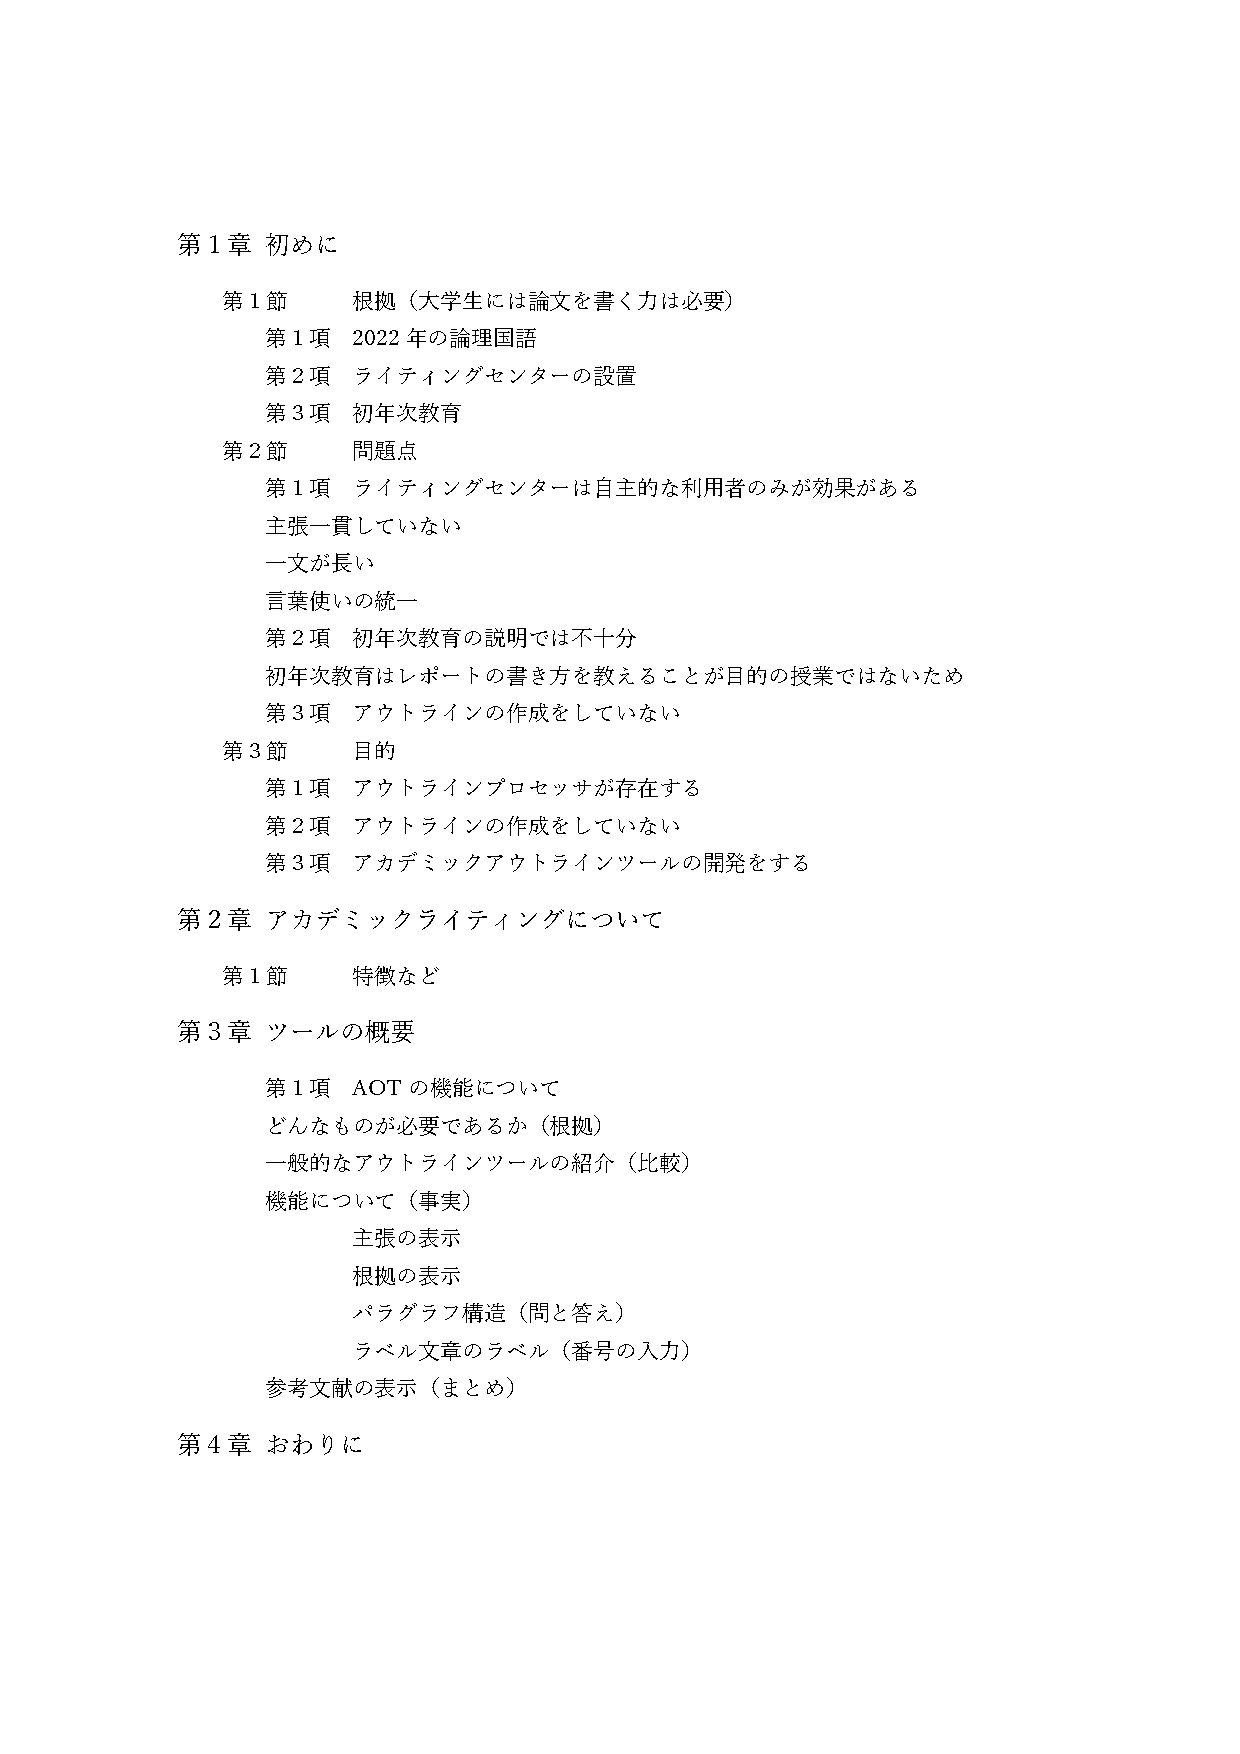
\includegraphics[scale=0.3]{outline.pdf}
\end{center}
 \caption{アウトラインの作成例}
 \label{fig:a}
\end{figure}
\newpage

\subsection{アカデミックライティングとは}
アカデミックライティングとは大学で作成が求められる,レポートや卒業論文や研究学術論文などの学術的な文章を書く技術または行為のことを指す\cite{ren2}.
\subsection{特徴}
アカデミックライティングには重要な特徴として,以下の(1)〜(5)が挙げられる.
\begin{description}
  \item[(1)] 主張と根拠が明示されている
  \item[(2)] 問いと答えの構造と論理的な説明での構成されている
  \item[(3)] 引用の倫理のルールに従っている
  \item[(4)] パラグラフ構造になっている
  \item[(5)] 学術的文章に特有の一定の形式に従ってる
 \end{description}

\newpage
\section{論文などの作成を支援するソフトウェアの紹介}
本章では論文などの作成を支援するソフトウェアを紹介する.
\subsection{アウトラインプロセッサ}
アウトラインプロセッサとは,一般的には小説などの長文を書く際に利用されている.
特徴として,見出しをつけ階層的に管理や位置の入れ替えなど行い,全体の構成を確認しながら文章の作成を支援するソフトウェアである.
\subsection{TEX}

\subsection{Microsoft Word}

\subsection{マインドマップ}

\newpage
\section{実装技術}
\subsection{PWA}
\newpage
\section{本研究で開発したツールの概要}
\subsection{実装理由}
%実装した機能がなぜひつようであるのか?コンセプトを書く
\subsection{開発言語}
\subsection{実装した機能について}
\subsubsection{主張と根拠の明確化}
\subsubsection{課題に対する疑問とその答えの記入}
\subsubsection{論理的な構成の整理}
\subsubsection{参考文献の管理}

\subsection{利用方法}

\newpage

\section*{謝辞}

\addcontentsline{toc}{section}{謝辞}
ここに研究の謝辞.主にご協力いただいた方など.
\bibliographystyle{jplain}
\newpage
\addcontentsline{toc}{section}{参考文献}
 \begin{thebibliography}{99}
\bibitem{ren1}山崎 憲一,萬代 雅希"論文とは",電子情報通信学会 通信ソサイエティマガジン,2016年9巻4号216-221.
\url{https://www.jstage.jst.go.jp/article/bplus/9/4/9_216/_pdf}

\bibitem{ren2} 堀 一成,坂尻 彰宏:"阪大生のためのアカデミックライティング",
\url{https://ir.library.osaka-u.ac.jp/repo/ouka/all/27153/Academic%20Writing%20Introduction.pdf}, 2019/8/23参照
\end{thebibliography}

\section*{付録}

\addcontentsline{toc}{section}{付録}

\end{document}
